\documentclass[../masterarbeit.tex]{subfiles}
\begin{document}
	














\subsection{Machine Learning}
The initial idea behind all artificial intelligence concepts is to make a computer able to perform tasks, that normally have to be accomplished by human brains. Machine learning is a subfield of artificial intelligence wich became popular in the 1990s and is inspired by theories from psychology and neuroscience about how humans learn. \autocite[]{VIEIRA20201} \autocite[]{SUBASI202091}
Abdulhamit Subasi describes the initial goals of machine learning in his book "Practical Machine Learning for Data Analysis Using Python" as follows:
\begin{quote}
	"The goals of machine learning are defined as development and improvement of
computer algorithms and models to meet decision-making needs in real-world situations." \autocite{SUBASI202091}
\end{quote}
Machine learning models are supposed to recognize patterns within data based on learning data in order to be able to make predictions or decisions based on their findings in combination with new or unseen data. They are algorithms designed to automatically improve their decisions and predictions based on experience. Additional information should therefore help them make better predictions. The models learn rules wich are generalizable, since it is not very likely that the model makes predictions on exactly the same data, but in most cases receives similar data for that process. \autocite[]{VIEIRA20201}
One of the biggest obstacles in the field of machine learning is obtaining good data, because ultimately the quality of the model depends directly on the quality of the data. Data acquisition can be very time-consuming and difficult, as there are no high-quality data sets for many scenarios. \autocite[]{SUBASI202091}
\begin{figure}[h]
    \centering
    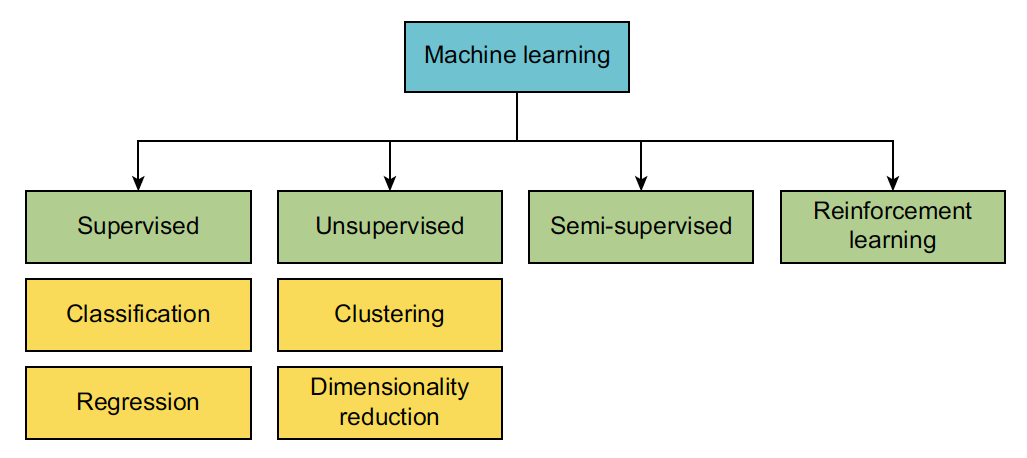
\includegraphics[scale=0.4]{machine_learning.png}
    \source{\autocite[]{PISNER2020101}}
    \caption{Machine learning model learning types.}
\end{figure} \\
As shown in figure 3, in Machine learning there are four base types of models: supervised, unsupervised, semisupervised and reinforcement learning. \autocite[]{VIEIRA20201} \autocite[]{ibm-supervised-learning:2022} \autocite[]{PISNER2020101}
 \\~\\
Supervised learning models get their names from the fact, that they are knowing both input and output variables during learning process. Therefore, they know the output values they are supposed to predict. They try to recognize the best possible relationship between input and output values while being trained on examples. Labeled datasets are used to train this models. During the training process, the weighting of the features is adjusted until the model is well fitted to the data set. \autocite[]{VIEIRA20201} \autocite[]{ibm-supervised-learning:2022}
As a comparison for the way a supervised learning model learns with humans, the authors Sandra Vieira and Walter Hugo Lopez Pinaya and Andrea Mechelli use in their book "Machine Learning" the way a student learns from his teacher. The teacher knows the right answers, asks the student questions, and gives feedback on the student's answers. \autocite[]{VIEIRA20201}
As illustrated in figure 3 supervised learning is divided into two subcategories, classification and regression. \\~\\
The machine learning algorithms wich are used for classification attempt to identify the relationship between the features of an observation and, on the basis of this, assign the observation to one of a number of classes, wich are known in advance \textcite[]{VIEIRA20201} \textcite[]{SUBASI202091}. For example, the two classes that are in the context of this work are: "an avalanche is going down" and "no avalanche is going down". 
While the classes in classification are fixed in advance, in regression any real numeric value on a continuous scale can be used for the prediction. The output variable is therefore not a categorical but a continuous one. \autocite[]{VIEIRA20201} \autocite[]{SUBASI202091} \\
The sustainable use of supervised learning models can be challenging, since a certain level of expertise is required for their use, training the models can be time-consuming, erroneous records may have already been made when the dataset was created, and the algorithms cannot independently classify or cluster the dataset but rely on predefined classifications or regressions \textcite[]{ibm-supervised-learning:2022}. \\~\\
In contrast to supervised learning, there is no target value to be predicted in unsupervised learning; the learning process is reduced to the structures within the data. Thus, the main applications of this type of learning are clustering, where similar data points are recognized and clustered based on the structures within the data, and the second is dimensionality reduction, wich is used to reduce the dimensionality of a dataset if the number of features is higher or near to the number of rows in the dataset.\autocite[]{ibm-supervised-learning:2022} \autocite[]{VIEIRA20201} \\~\\
Semi-supervised learning is an addition to supervised learning. It is used in cases of partly labeled datasets and makes it possible to integrate the unlabeled data into a supervised learning. \autocite[]{ibm-supervised-learning:2022}\autocite[]{VIEIRA20201}
The reinforcement machine learning algorithms are used to learn from interactions with their environment. So in the beginning there is no dataset needed to train this type of machine learning algorithms. The learning methodology behind these algorithms is based on the concept of rewards and punishments that it receives based on its decisions, and attempts to arrive at as many rewards and as few punishments as possible in the course of learning based on trail and error. Compared to supervised learning, the algorithm is free in its behavior in the reinforcement technique. \autocite[]{ionos-reinforcement-learning:2022} \autocite[]{VIEIRA20201} \\~\\
In order to achieve adequate results, a series of machine learning models are trained in the context of the thesis. Causing the fact that the prediction of avalanches for explizit defined locations is a binary classification problem, only machine learning models of the supervised learning type are applied on the task.\\
In the past, some models have already proven their worth in predicting natural disasters. For example, the Support Vector Machine (SVM) and the Multivariate Discriminant Analysis (MDA) models, wich is an addition to the Linear Discriminant Analysis described in chapter 3.2.3. They are useful for detecting subtle patterns in complex data sets and Flexible in handling data of different dimensions. SVM models are designed to deal with high dimensional data. Thats one aspect why they have already been used to predict natural disasters, such as earthquakes, floods, typhoons, drought, landslides and avalanches \textcite[]{Bahram:2019} \textcite[]{Tiwari:2021} \textcite[]{Pozdnoukhov:2008}. MDA forms efficient linear combinations of independent variables. MDAs have not been used that often to predict natural disasters, but shows superior performance compared to SVM in the case study in the Karaj water conservation area in predicting avalanche risk levels \textcite[]{Bahram:2019}. So for this master thesis a logistic regression, support vector machine and a multivariate discriminant analysis are trained, evaluated and the performance compared. The three machine learning models Logistic Regression, Support Vector Machine and Linear Discriminant Analysis are all relatively transparent about their approach to predicting observations. The three models are described in the next three chapters in detail.


\subsubsection{Logistic Regession}

The Logistic Regression is a popular classification training algorithm, wich is often used in the field of predictive analytics. It is also a supervised and discriminative machine learning model. \autocite[]{ibm-logistic-regression:2022} 
The logistic regression and linear regression models are two of the most popular models in the field of data science, as they are very easy to execute and require little computation time. linear regression is used to find the correlation between two features. This is done by drawing the line that best fits through a number of data points. While the method, wich is used by the linear regression to calculate the loss function, is the mean squared error, in logistic regression the maximum likelihood estimation is used. Similar to the behavior of the linear regression, logistic regression is used to calculate the correlations between one or multiple features and the variable to be determined, but it is used to predict categorical variables.  Binary categorical variables can only have two states, for example 1 or 0. So because lineare regression is used to predict continuous variables the major difference between them is, that logistic regression handles binary classification problems and linear regression handles the regression problem. \autocite[]{BELYADI2021169} \textcite[]{ibm-logistic-regression:2022} \textcite[]{Sourav:2020} The name "Logistic regression" can be misleading, because it is more a classification model than a regression model \textcite[]{SUBASI202091}. Instead of directly searching for the best fitting regression line in the data, like the lineare regression model does, it splits this process into three steps. First, similar to the linear regression, a regression line is fit onto the data. In the case of predicting categorical variables, the line is very susceptible to outliners. Because of that fact the next step is to feed the results to the sigmoid function, wich outputs are always between 0 and 1. \autocite[]{ibm-logistic-regression:2022} \textcite[]{Sourav:2020} \textcite[]{BELYADI2021169}\\
The sigmoid function also known as logistic function: \\~\\
\( S(x) = \frac{1}{1 + e^{-x}}\) \hfill \textcite[]{Sourav:2020} \textcite[]{BELYADI2021169} \\~\\
As a last step the result values of the sigmoid function are converted to the values 0 or 1 (discrete values) based on the threshold, wichs standard value is 0.5. This means if the value is greater than 0.5 the resulting prediction value is turned to 1 and if it is smaller it is changed to 0. \autocite[]{Sourav:2020} \textcite[]{BELYADI2021169}
\begin{figure}[h]
    \centering
    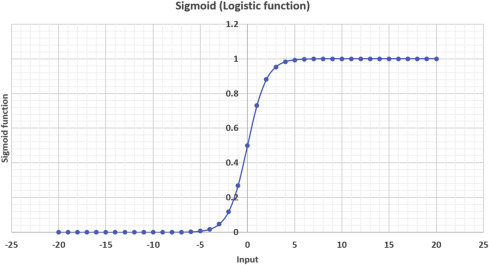
\includegraphics[scale=1]{logisticRegression.jpg}
    \source{\autocite[]{BELYADI2021169}}
    \caption{Sigmoid function curve in logistic regression.}
\end{figure} \\
The S-curve displayed in figure 4 is the result of the sigmoid function fed with values between -20 and 20. As the curve shows, the values resulting from the logistic function are in the range between 0 and 1.\\
In addition to the binary classifications variant, which is the most widely used variant of logistic regression and generally one of the most common methods for binary classification, there are two other variants. The Multinomial logistic regression and the Ordinal logistic regression. The Multinomial logistic regression is used for classification with three or more possible result values for the determined value, wich are in no particular order. Ordinal logistic regression is also used for multiclass classification tasks, but in this case the variables are in a specific order. For example a evaluation scalar with one to five stars. \autocite[]{ibm-logistic-regression:2022} \textcite[]{SUBASI202091} \\
Similar to other machine learning models, like neuronal networks, support vector machines and multiple discriminant analysis, wich are also used in context of this master thesis and described in detail in the later part of the work, logistic regression does not need linear relations between the predictor variables and the variable to be determined. They capture nonlinear relationships in the dataset. \autocite[]{NUSINOVICI202056} \textcite[]{BELYADI2021169} \\
Logistic regression models are easy to realize while they are achieving good results for binary and linear classification problems \textcite[]{SUBASI202091}. For Example V. Sugumaran, V. Muralidharan and K.I. Ramachandran found out, that for their case study about major chronic diseases logistic regression could keep up with the other machine learning algorithms and in two cases even delivered better results \textcite[]{NUSINOVICI202056}.
The Python library Scikit-learn does have a optimized version of the logistic regression algorithm, wich also can handle dens as well as sparse input by including a set of regularization methods to convert any format to 64-Bit floats for the optimal performance of the algorithm\textcite[]{Scikit-learn-logistic-regression:2022}. In context of this thesis, the scikit-learn implementation is used.



\subsubsection{Support Vector Machine}

Support Vector Machines (SVM) are supervised machine learning algorithms based on the statical learning theory and have been introduced the first time in the 1990s and developed by Vladimir Vapnik \textcite[]{ibm-supervised-learning:2022} \textcite[]{SUGUMARAN2007930} \textcite[]{GHOLAMI2017515}. They can be used for classification and regression problems as well as to detect outliners \textcite[]{ibm-supervised-learning:2022} \textcite[]{Scikit-learn-svm:2022}.
Abdulhamit Subasi gives a general overview about SVMs in his book "Practical Machine Learning for Data Analysis Using Python" as follows:
\begin{quote}
	"Support vector machines (SVMs) are one of the main machine-learning algorithms that are not only accurate but also highly robust." \autocite{SUBASI202091}
\end{quote} 
The method, wich Support Vector Machines use, tries to find the best classification function that splits the training set into the classes of the variable to be determined. \autocite[]{SUBASI202091}
Each feature can also be considered as a dimension in a hyperspace. The SVM creates a hyperplane to split the hyperspace into two or more parts. This depends on how many classes are to be predicted.
So the SVM can be applied to cases of the multi-class problem just like decision trees. \autocite[]{SUGUMARAN2007930}
Support vector machines can be linear and non-linear, but classification problems are in most cases linear, therefore mostly linear SVMs are in use \textcite[]{PISNER2020101}. \\
If the data is not linearly separable, the support vector machine can not create a good generalization. To solve this problem, it projects the data points onto a higher dimensional hyperspace. Based on the mathematical assumption that a non-linear separation in a higher dimensional space is linear. This higher dimensional space is also called Hilbert or feature space. As a result of this assumption, the input data are still non-linear, but in the feature space the application of a linear Svm and thus a better generalization is possible. Figure 5 displays the differences between the input space and the higher dimensional feature space, in wich a linear hyperplane is placed to separate the data. \autocite[]{GHOLAMI2017515} \\
\begin{figure}[h]
    \centering
    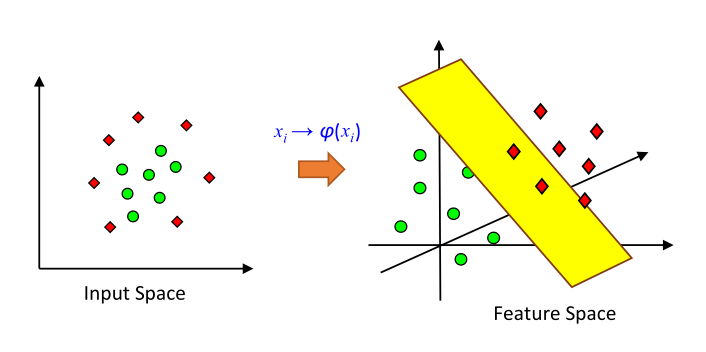
\includegraphics[scale=0.5]{input_space_feature_space_svm.png}
    \source{\autocite[]{GHOLAMI2017515}}
    \caption{Input space in comparison to higher dimensional feature space.}
\end{figure}
\\
In the case that the data set is linearly separable, the linear function is used to compare the separating hyperplanes. This is necessary because in this case the SVM raises the margin between the classes to the maximum based on these quantities. Contrary to the assumed definition that margin is the space between classes, the mathematical definition is the shortest distance from the hyperplane to the closest data point. Although many hyperplanes are located in hyperspace, support vector machines can only use two of them. To ensure the best possible classification of current and future data, the most extreme margin of the hyperplanes is determined. \autocite[]{SUBASI202091}
The search for the maximum margin is minimizes also the generalization error of the SVM. \autocite[]{SUGUMARAN2007930} \\
A larger margin allows better generalization and a hard margin is the simplest way with the least computation time, but it might not be perfect in practice. In fact that, in the case of a hard marin, the hyperplane is affected even by one single outliner. This lead to hyperplane mistakes and misclassification. So another option is to use a soft margin instead. In this approach the hyperplane can get highly complex so as a compromise the penalty factor C, wich is called the "soft margin constant" comes into the process. It is used to make a compromise between complexity and classification errors as well as reducing the chance of overfitting. For this reason, it is often argued that the soft margin variant should also be used for linearly separable datasets. \autocite[]{PISNER2020101} \textcite[]{GHOLAMI2017515} \\
Support vector machines can also be used for the generalization and are effective for highly distributed, high dimensional or spare datasets, even if the number of samples is smaller than the number of dimensions. It also indicates an higher accuracy in comparison to other classification machine learning methods like Neuronal Networks, because of its good generalization capacity. \autocite[]{SUBASI202091} \textcite[]{Scikit-learn-svm:2022} 

As shown in Section 2 "Related Work", SVMs performed well in previous studies in the context of avalanche event prediction and avalanche hazard mapping. \autocites[]{Tiwari:2021, THURING201560, Bahram:2019, Pozdnoukhov:2008}
In the context of this work one implementation included in the Python library Sklearn.svm is used to build the prediction model. The chosen algorithm is called C-Support Vector Classification (SVC) \textcite[]{Scikit-learn-svc:2022} . The implementation of this algorithm is based on another Python library with the name libsvm, wich implements a series of different SVM algorithms. This implementation scales in the computation time at least quadratically. The documentation therefore mentions that the long computation time can be impractical when the number of samples exceeds 10000 and that another implementation, such as LinearSVC, should be chosen in that case. \autocite[]{Scikit-learn-svc:2022}
In the case of this study, however, the number of samples is less than 10000 and the implementation can be used.




\subsubsection{Linear Discriminant Analysis}


Linear Discriminant Analysis (LDA) is a fundamental data analysis method, wich has been first time examined by Fisher in 1936 for two classes and later in 1948 C.R. Rao found it for multiple classes \textcite[]{DEMIR2005421} \textcite[]{analyticsvidhyaLDA:2021} \textcite[]{Xanthopoulos2013}. R. Fisher used the LDA to differenciate between two different types of plants \textcite[]{Xanthopoulos2013}. 
LDAs are supervised machine learning algorithms, as it depends on user input and the knowledge about class affiliation of each data point, but it is also a dimensionality reduction techinque. For this reason it can be used as classifier machine learning method to classify samples of an dataset with multiple independent variables to two or more classes and also to determine the class of unknown varibales. It can also be used for data preprocessing as a dimension reducing method or to identify the how significant the individual features are, represented by the corresponding coefficients of the hyperplane.  \autocite[]{MENDLEIN2013646} \autocite[]{Bahram:2019} \autocite[]{Xanthopoulos2013} \autocite[]{SUBASI202091} \autocite[]{analyticsvidhyaLDA:2021}. 
Discriminate Analysis projects the data points as close as possible to the data points belonging to the same class and moves the individual classes as far away from each other as possible. This is done by defining the distance of the points from the center of their class, wich is calculated by the use of normal distribution. \autocite[]{MENDLEIN2013646} \autocite[]{Bahram:2019} \autocite[]{SUBASI202091} \autocite[]{Xanthopoulos2013}
Linear Discriminant Analysis increase the variability between the classes and reducing the variability within them by projecting the data from a \(D\) dimensional feature space on a lower dimensional subspace \(D'\) and creating new discriminant axes that represent linear combinations of the individual variables \textcite[]{analyticsvidhyaLDA:2021} \textcite[]{DEMIR2005421}. As an example Figure 6 shows  the projection of datapoints in da two dimensional space onto a lower dimensional subspace.\\
\begin{figure}[h]
    \centering
    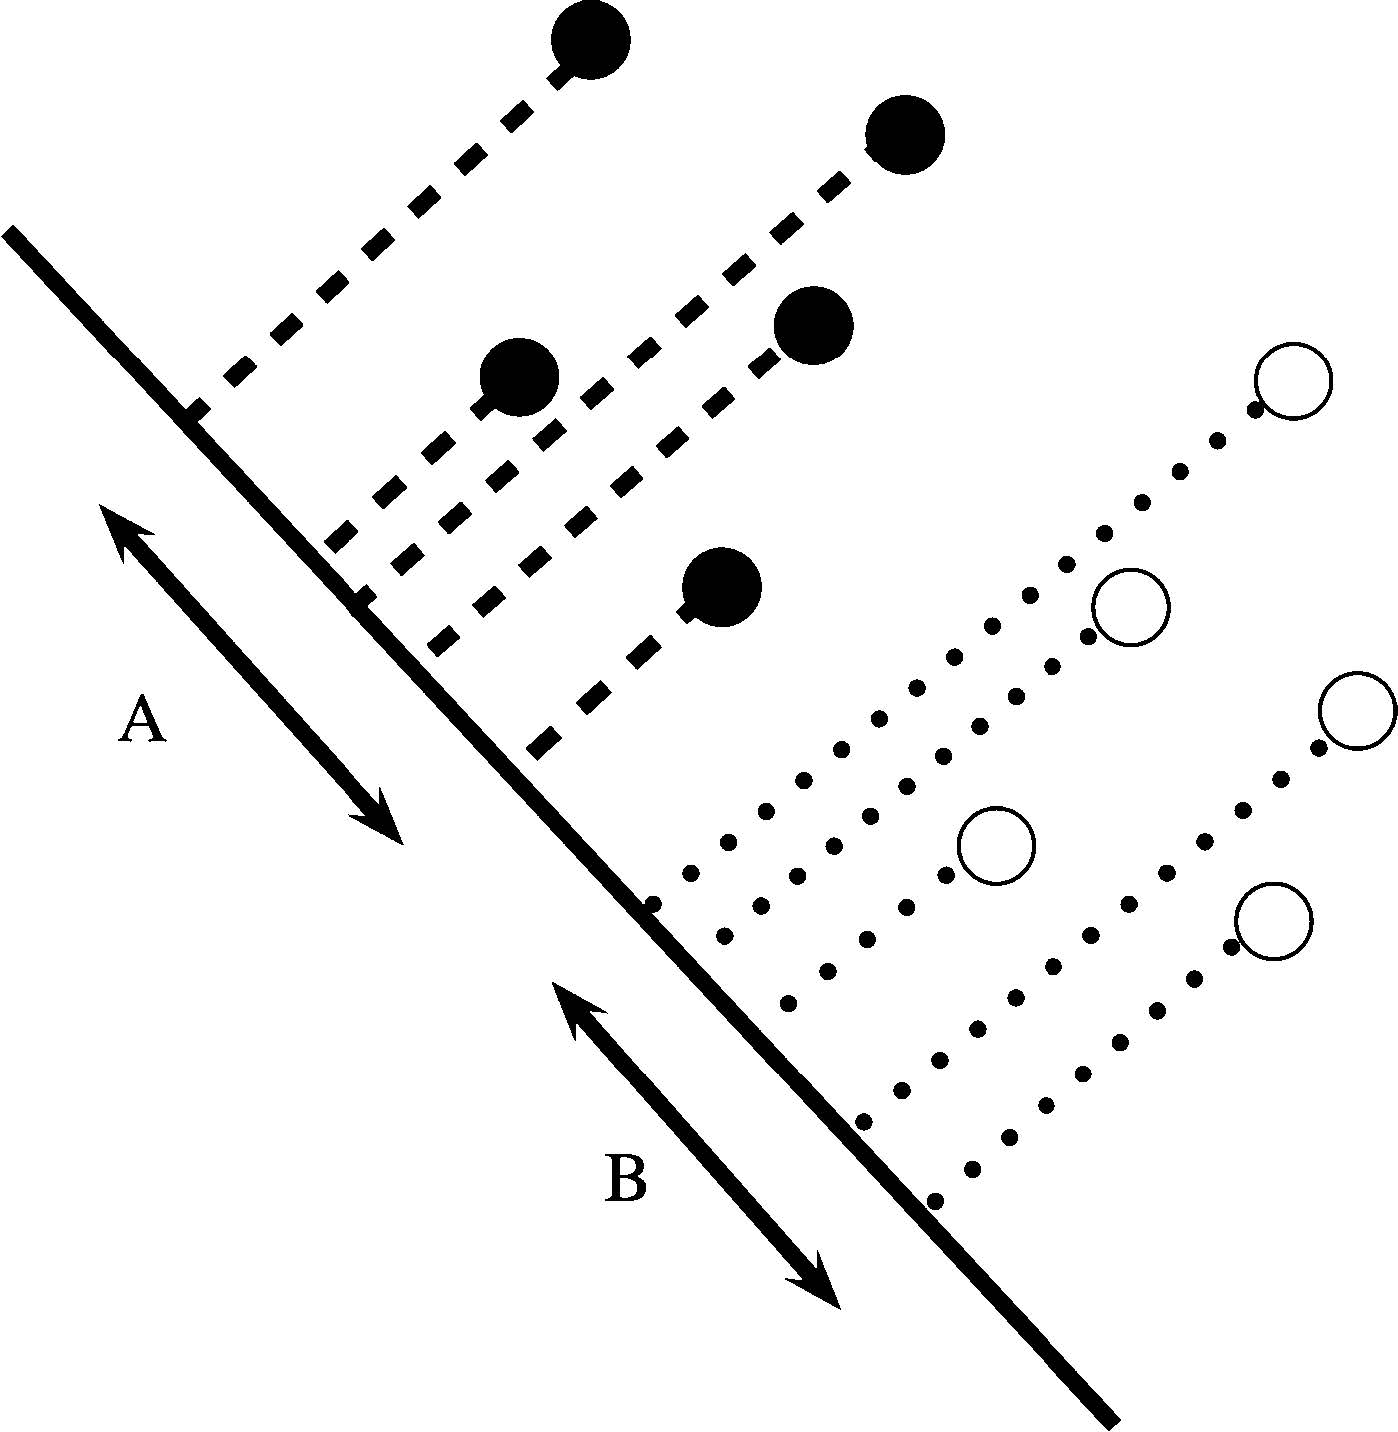
\includegraphics[scale=1.0]{two_dimensions_to_one.jpg}
    \source{\autocite[]{Xanthopoulos2013}}
    \caption{A Two dimensional data set is projected in a lower dimensional subspace, wich is a line. In this way the separability is increased.}
\end{figure} 
This process consists of three steps. At first, the separability between the classes needs to be calculated. It represents the distance between the mean of one class to the mean of another one and is called the "between-class variance". This variance is calculated for every class and a between class matrix \(S_B\) is created. The between-class variance for the \(i\)th class \(S_{B_i}\) is the distance of the class mean \(\mu_i\) and the total mean \(\mu\). \autocite[]{Tharwat:2017} \\
In the second step, the distances of the individual data points within a class, also known as the "within-class variance", are calculated. The within-class variance \(S_{W_i}\) is calculated based on the distance from each point within a class with the mean of the class. \autocite[]{Tharwat:2017} \\
In the last step, the lower dimensional subspace is constructed so that the between-class variance is as large as possible and the within-class variance is as small as possible. For this step, there are two methods for the calculation of the lower dimensional subspace. In the first one, wich is class-dependent, a lower dimensional subspace is generated for every class and project its data points onto it. The second method is called class-independent. It only calculates one subspace for all classes and projects their data points on it. \autocite[]{Tharwat:2017}
\begin{figure}[h]
    \centering
    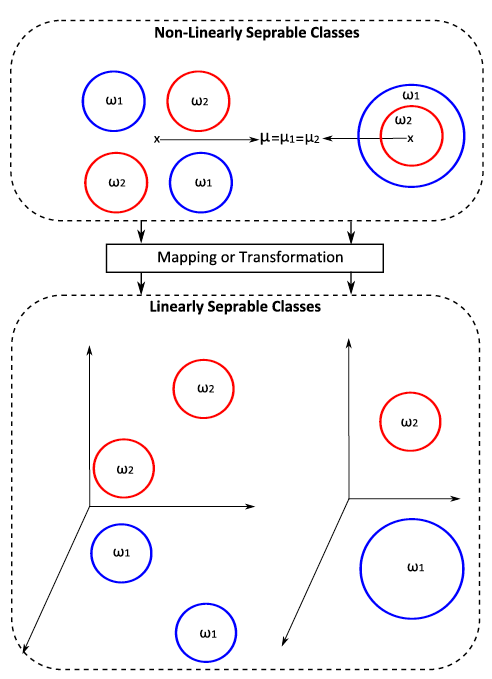
\includegraphics[scale=0.5]{non-linearly_LDA.png}
    \source{\autocite[]{Tharwat:2017}}
    \caption{Two different examples for non-linear separable classes, in wich the problem is solved by generating a higher dimensional space and make a linear separation of the classes possible for the LDA.}
\end{figure} \\
LDAs do have two main problems. The Small Sample Problem and the linearity problem.
The Small Sample Problem means that LDAs can not handle datasets where the number of variables is larger than the number of samples. This would cause a fail calculation of the lower dimensional subspace by the LDA. \autocite[]{MENDLEIN2013646} \autocite[]{analyticsvidhyaLDA:2021} \autocite[]{Tharwat:2017}
The LDA can also run into another problem, the "linearity problem". This problem arises when the individual classes are non-linearly seperable. In this case the LDA fails to find a lower dimensional subspace. For example when the means of the classes are equal. One approach to fix this problem is to create a higher dimensional space, similar to the svm. An example for this scenario and how the problem is solved by increasing the dimensions of the space is shown in figure 7. The four datapoints in the figure are not linearly separable on the two dimensional space and the problem does not get solved by putting it onto a lower dimensional subspace. So the LDA projects them onto a three dimensional space. In this new higher dimensional space the classes are linearly separable and can be projected onto a lower dimensional subspace. \autocite[]{Tharwat:2017} \\
The Multivariate Discriminant Analysis (MDA), wich is an addition to the LDA, has brought good results in a study in the Karaj watershed, in wich they used SVMs and MDAs for an avalanche hazard prediction and compared the performance of both algorithms \textcite[]{Bahram:2019}. \\
For the case study of this master thesis the Python implementation of Linear Discriminant Analysis, wich is included in the library sklearn.discriminant\_analysis is used. \autocite[]{Scikit-learn-lda:2022}
















\end{document}
